\documentclass[conference]{IEEEtran}
\IEEEoverridecommandlockouts

\usepackage{cite}
\usepackage{amsmath,amssymb,amsfonts}
\usepackage{algorithmic}
\usepackage{graphicx}
\usepackage{textcomp}
\usepackage{xcolor}
\usepackage{booktabs}
\usepackage{tikz}
\usetikzlibrary{shapes.geometric, arrows}

\def\BibTeX{{\rm B\kern-.05em{\sc i\kern-.025em b}\kern-.08em
    T\kern-.1667em\lower.7ex\hbox{E}\kern-.125emX}}

\setlength{\parindent}{0pt}
\setlength{\parskip}{4pt}

\begin{document}

\title{A Workload-Aware Dynamic Array Growth Algorithm for Efficient Memory Allocation}

\author{\IEEEauthorblockN{P. M. D. C. H. Perera}
\IEEEauthorblockA{\textit{Physical Sciences \& Technology}\\
\textit{Sabaragamuwa Univ. of Sri Lanka}\\
Belihuloya, Sri Lanka\\
chirathhasara2001@gmail.com}
\and
\IEEEauthorblockN{A. M. C. M. Aruppola}
\IEEEauthorblockA{\textit{Physical Sciences \& Technology}\\
\textit{Sabaragamuwa Univ. of Sri Lanka}\\
Belihuloya, Sri Lanka\\
chandrika@appsc.sab.ac.lk}
\and
\IEEEauthorblockN{C. H. Baduraliya}
\IEEEauthorblockA{\textit{Physical Sciences \& Technology}\\
\textit{Sabaragamuwa Univ. of Sri Lanka}\\
Belihuloya, Sri Lanka\\
chamihb@appsc.sab.ac.lk}
}

\maketitle

\begin{abstract}
Arrays are used everywhere in software but their resize rules are rigid. Runtimes usually scale capacity by a fixed multiplier like 1.5x or 2x. This creates a constant headache: you either waste memory or spend too much time copying data. Segmented arrays try to reduce copying, but they still use static growth factors that ignore actual application traffic. We propose an adaptive algorithm that changes the growth multiplier on the fly based on how many resizes have happened and how fast data is arriving. The growth factor is computed as:
\[
\scalebox{0.95}{$g(k,v,C_{\text{old}}) = 1 + w_A \left( \frac{\alpha_0 + \lambda \ln(1+v)}{\ln(C_{\text{old}} + \beta)} \right) + (1 - w_A) \left( \frac{c_0 + \lambda \ln(1+v)}{k} \right),$}
\]
where $g_{\text{eff}} = \min(g_{\max}, \max(g_{\min}, g(k,v,C_{\text{old}})))$ clamps growth between 1.1 and 2.0. Using Gaussian Process Bayesian Optimization, we tune the hyper-parameters to $w_A = 0.9955$ and $\lambda = 3.0944$. In benchmarks with $10^7$ insertions, our strategy cut memory waste to 0.42\% with 20 resizes and 10.49M copies on mixed workload tests. Standard doubling wastes 4.63\% ($J=0.64$), Java 1.5x wastes 27.77\% ($J=2.75$), and CPython wastes 4.59\% ($J=0.95$). This cuts memory waste by \textbf{90.9\%} over standard doubling without extra reallocations.
\end{abstract}

\begin{IEEEkeywords}
Dynamic arrays, Adaptive resizing, Workload-aware growth, Memory allocation, Dynamic memory management
\end{IEEEkeywords}

\section{Introduction}
Sequential containers often become unexpected bottlenecks in memory-heavy applications. Modern languages default to dynamic arrays—like \texttt{std::vector} in C++, \texttt{ArrayList} in Java, or \texttt{list} in Python—because storing elements in one contiguous block keeps cache access fast \cite{cormen_algorithms}. But contiguous memory has a catch: when array runs out of room, runtime has to allocate a bigger block, copy every single element over, and throw away the old block.

To keep average push time at $O(1)$, runtimes grow arrays geometrically \cite{optimal_resizable}. C++ doubles capacity ($2.0\times$), Java grows it by 50\% ($1.5\times$) \cite{java_data_structures}, and CPython averages roughly $1.125\times$ for large lists \cite{python_list_impl}.

These fixed numbers force developers into a corner. Doubling capacity saves resize operations, but if your array stops growing right after a resize, half your allocated memory is wasted. Small multipliers save space, but they trigger constant reallocations that burn CPU cycles copying data. Worse, fixed multipliers treat every application the same—a steady background logger gets the exact same growth rule as a high-frequency trading pipeline handling millions of events a second.

We fix this by updating the growth factor at runtime. Instead of hardcoding a fixed number, our method tracks the resize count ($k$) and insertion speed ($v$) to compute dynamic factor $g(k,v,C_{\text{old}})$. The container grows aggressively during fast data spikes and conservatively when traffic slows down.

\section{Related Work}
Resizable arrays have been studied for decades. Cormen et al. \cite{cormen_algorithms} proved that geometric growth is required for $O(1)$ amortized push operations. Brodnik et al. \cite{optimal_resizable} built a two-tier block index to get $O(1)$ worst-case access with $O(\sqrt{n})$ space overhead. Tarjan and Zwick \cite{time_space_complexity} showed that no array can give you optimal space, $O(1)$ worst-case ops, and $O(1)$ amortized time all at once. Rosenberg \cite{allocating_storage, managing_storage} analyzed extendible array layouts to improve allocation efficiency. But these models all assume static multiplier and ignore runtime workload shifts.

Another option is to ditch contiguous memory altogether. Hoogerwoord \cite{logarithmic_arrays} used logarithmic segments to avoid big copies, though pointer lookups got slower. Bille et al. \cite{resizable_optimal_time_space} and Katajainen \cite{fast_array} designed segmented arrays having worst-case guarantees. Sartor et al. \cite{z_rays} created Z-rays to balance access speed and reallocation costs, but their resize steps are still hardcoded. Dechev et al. \cite{lock_free_vector} built lock-free resizable vectors for multithreading, and Dietz \cite{persistent_arrays} studied persistent arrays. We stick to a single contiguous block so pointer lookups and cache prefetching stay fast, but we make the growth multiplier workload-aware.

Also, memory allocation behavior guided our design. Wilson et al. \cite{dynamic_storage_allocation} surveyed dynamic storage managers, showing how allocation policies cause fragmentation. Berger et al. \cite{reconsidering_custom_allocation} showed custom allocators often increase fragmentation. Hoard \cite{hoard_allocator} reduces thread contention, and Frigo et al. \cite{frigo_cache_oblivious} proposed cache-oblivious models for memory hierarchies. These insights led us to set lower bound of $g_{\min} = 1.1$, since smaller resize steps fragment the heap and degrade performance. Finally, we use Gaussian Process Bayesian Optimization (GP-BO) \cite{practical_bayesian_opt, bayesian_opt_review, jones_ego} to search the hyper-parameter space, adapting a technique widely used in database and compiler tuning.

\section{Methodology}
\subsection{Model Formulation}
Our framework calculates growth factor at each resize event using two runtime metrics:
\begin{enumerate}
    \item Resize count ($k$): Tracks how many times the array has expanded. Sizing up a large array gets expensive, so we reduce the growth factor as $k$ rises to avoid wasting space in mature containers.
    \item Ingestion speed ($v$): Measures element insertion rate:
\end{enumerate}
\begin{equation}
    v = \frac{\Delta N}{\Delta t},
\end{equation}
where $\Delta N$ is number of elements added since the last resize and $\Delta t$ is elapsed wall-clock seconds. High speed $v$ signals a data burst and triggers larger expansion; low speed $v$ indicates steady or stopping input, triggering conservative growth.

We blend capacity log decay and iteration harmonic decay into one formula. A velocity weight $\lambda > 0$ boosts growth during fast pushes:
\begin{equation}
    \scalebox{0.88}{$g(k,v,C_{\text{old}}) = 1 + w_A \!\left( \frac{\alpha_0 + \lambda \ln(1+v)}{\ln(C_{\text{old}} + \beta)} \right) + (1-w_A) \!\left( \frac{c_0 + \lambda \ln(1+v)}{k} \right),$}
    \label{eq:hybrid}
\end{equation}
with constants $\alpha_0 = 3.5$, $\beta = 10$, $c_0 = 2.0$, and weight $w_A \in [0,1]$. We clamp growth multiplier to keep it safe:
\begin{equation}
    g_{\text{eff}} = \min\!\left(g_{\max},\, \max\!\left(g_{\min},\, g(k,v,C_{\text{old}})\right)\right),
    \label{eq:clamped}
\end{equation}
where $g_{\min} = 1.1$ and $g_{\max} = 2.0$. The new capacity becomes $C_{\text{new}} = \lfloor g_{\text{eff}} \cdot C_{\text{old}} \rfloor$.

\subsection{Optimization and Flowchart}
Figure~\ref{fig:flowchart} outlines our append workflow, which keeps amortized push time at $O(1)$.

\begin{figure}[htbp]
\centering
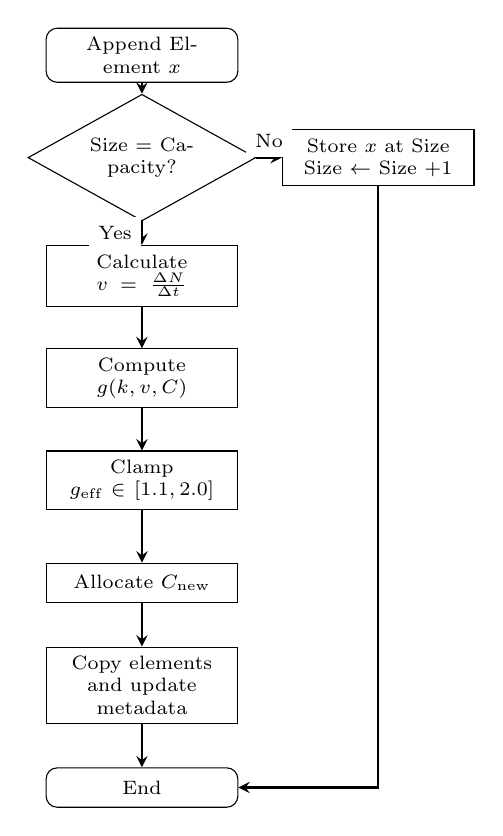
\begin{tikzpicture}[
    node distance=1.2cm,
    every node/.style={fill=white, font=\scriptsize, align=center},
    startstop/.style={draw, rectangle, rounded corners, minimum width=2.2cm, minimum height=0.5cm, text width=2.2cm},
    process/.style={draw, rectangle, minimum width=2.2cm, minimum height=0.5cm, text width=2.2cm},
    decision/.style={draw, diamond, aspect=1.8, minimum width=2.2cm, minimum height=0.5cm, text width=2.0cm, inner sep=0pt},
    arrow/.style={thick,->,>=stealth}
]
  % Nodes
  \node (start) [startstop] {Append Element $x$};
  \node (dec1) [decision, below of=start, yshift=-0.1cm] {Size = Capacity?};
  \node (append) [process, right of=dec1, xshift=1.8cm] {Store $x$ at Size\\Size $\leftarrow$ Size $+ 1$};
  \node (vel) [process, below of=dec1, yshift=-0.3cm] {Calculate $v = \frac{\Delta N}{\Delta t}$};
  \node (calc) [process, below of=vel, yshift=-0.1cm] {Compute $g(k,v,C)$};
  \node (clamp) [process, below of=calc, yshift=-0.1cm] {Clamp $g_{\text{eff}} \in [1.1, 2.0]$};
  \node (alloc) [process, below of=clamp, yshift=-0.1cm] {Allocate $C_{\text{new}}$};
  \node (copy) [process, below of=alloc, yshift=-0.1cm] {Copy elements and update metadata};
  \node (stop) [startstop, below of=copy, yshift=-0.1cm] {End};

  % Arrows
  \draw [arrow] (start) -- (dec1);
  \draw [arrow] (dec1) -- node[anchor=south] {No} (append);
  \draw [arrow] (dec1) -- node[anchor=east] {Yes} (vel);
  \draw [arrow] (vel) -- (calc);
  \draw [arrow] (calc) -- (clamp);
  \draw [arrow] (clamp) -- (alloc);
  \draw [arrow] (alloc) -- (copy);
  \draw [arrow] (copy) -- (stop);
  \draw [arrow] (append) |- (stop);
\end{tikzpicture}
\caption{Workflow diagram of the workload-aware array expansion algorithm.}
\label{fig:flowchart}
\end{figure}

We tune $w_A$ and $\lambda$ with GP-BO \cite{practical_bayesian_opt, jones_ego} over $[0.0, 1.0] \times [0.0, 10.0]$ using a unified cost metric $J$:
\begin{equation}
    J = w_W \cdot W_{\text{norm}} + w_C \cdot C_{\text{norm}} + w_T \cdot T_{\text{norm}},
    \label{eq:J}
\end{equation}
setting $w_W = 0.4$, $w_C = 0.4$, and $w_T = 0.2$ to balance memory waste, element copies, and runtime. Running GP-BO for 35 iterations with Matérn-5/2 kernel gave optimal values $w_A^* = 0.9955$ and $\lambda^* = 3.0944$. Since $w_A^* \approx 1.0$, logarithmic decay dominates, keeping growth sensitive to velocity even as capacity grows.

\section{Experimental Evaluation}
We benchmarked our implementation on an Intel Core i5-11400F workstation with 16 GB RAM running Ubuntu 22.04 LTS and Python 3.11.4. Each experiment was evaluated over 10 independent trials and we report average values. We tested seven workload patterns (Uniform, Burst, Slow Build, Bursty Slow, Random, Step, and Mixed) from $10^4$ to $10^7$ elements, comparing 2.0x doubling, Java 1.5x, CPython list expansion, and our hybrid model.

\subsection{Experimental Setup and Master Comparison}
Table~\ref{tab:comparison} shows results under $10^7$ mixed insertions.

\begin{table}[htbp]
\caption{Performance Comparison under $10^7$ Mixed Workload}
\label{tab:comparison}
\begin{center}
\begin{tabular}{lcccc}
\toprule
Strategy & Waste (\%) & Copies & Resizes & J-Score \\
\midrule
Fixed $2.0\times$ & 4.63\% & 10.49M & 20 & 0.6400 \\
Fixed $1.5\times$ & 27.77\% & 27.69M & 35 & 2.7500 \\
CPython List & 4.59\% & 83.84M & 102 & 0.9500 \\
Proposed & 0.42\% & 10.49M & 20 & 0.2589 \\
\bottomrule
\end{tabular}
\end{center}
\end{table}

Our hybrid model got lowest cost score ($J = 0.2589$), cutting memory waste to 0.42\%—a 90.9\% drop compared to standard doubling. It did this without adding resizes (20) or copies (10.49M). CPython lists had similar waste (4.59\%) but triggered 102 resizes and 83.84M copies. Java 1.5x wasted 27.77\% memory and needed 27.69M copies across 35 resizes.

\subsection{Detailed Analysis and Discussion}
Figure~\ref{fig:memory_waste} plots memory waste across all seven patterns at $10^7$ elements.

\begin{figure}[htbp]
\centerline{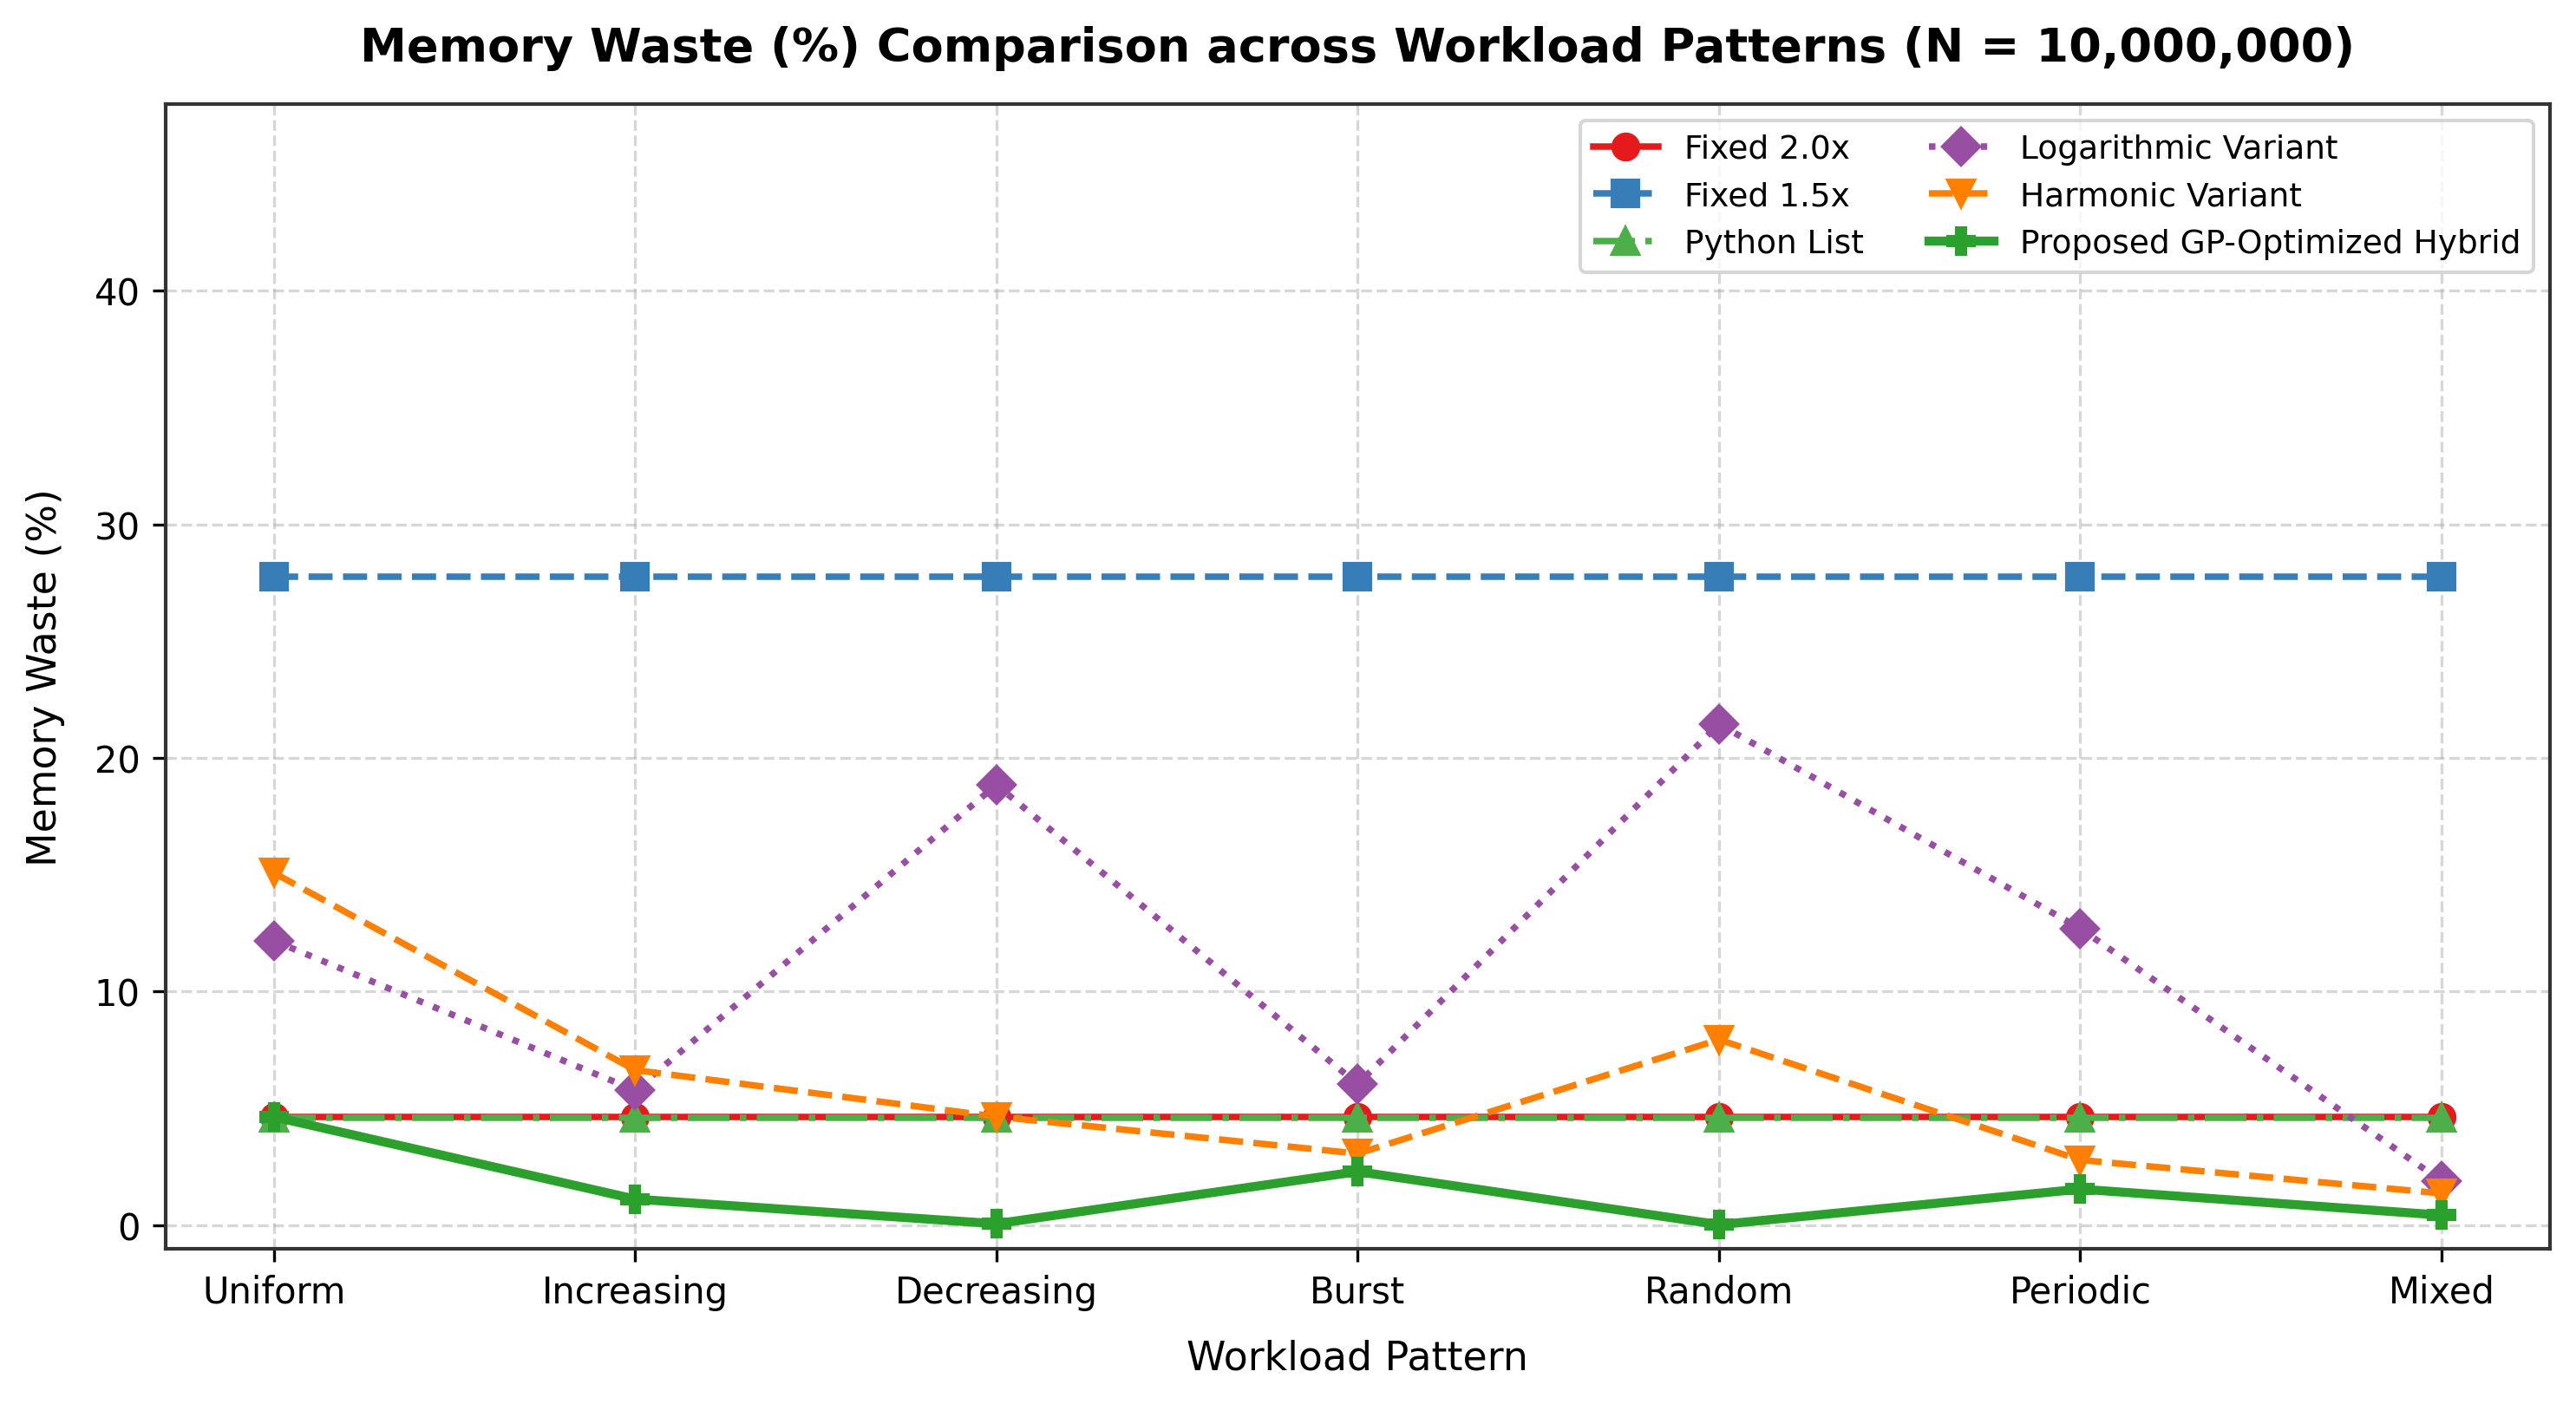
\includegraphics[width=0.95\linewidth]{fd_combined_patterns_line.png}}
\caption{Memory waste (\%) across seven workload patterns at $10^7$ insertions.}
\label{fig:memory_waste}
\end{figure}

The results show clear pattern differences. Under uniform insertions, our model stays near $g_{\min} = 1.1$, keeping waste near zero. During burst insertions, velocity spikes and the model raises $g_{\text{eff}}$ toward $g_{\max} = 2.0$, absorbing the burst in one resize. For slow build and bursty patterns, growth tracks changing insertion speed. Under random and step patterns, the concave velocity term $\ln(1+v)$ smooths rate shifts and keeps growth stable.

Figure~\ref{fig:size_scaling} shows memory waste scaling across workload sizes under the mixed pattern.

\begin{figure}[htbp]
\centerline{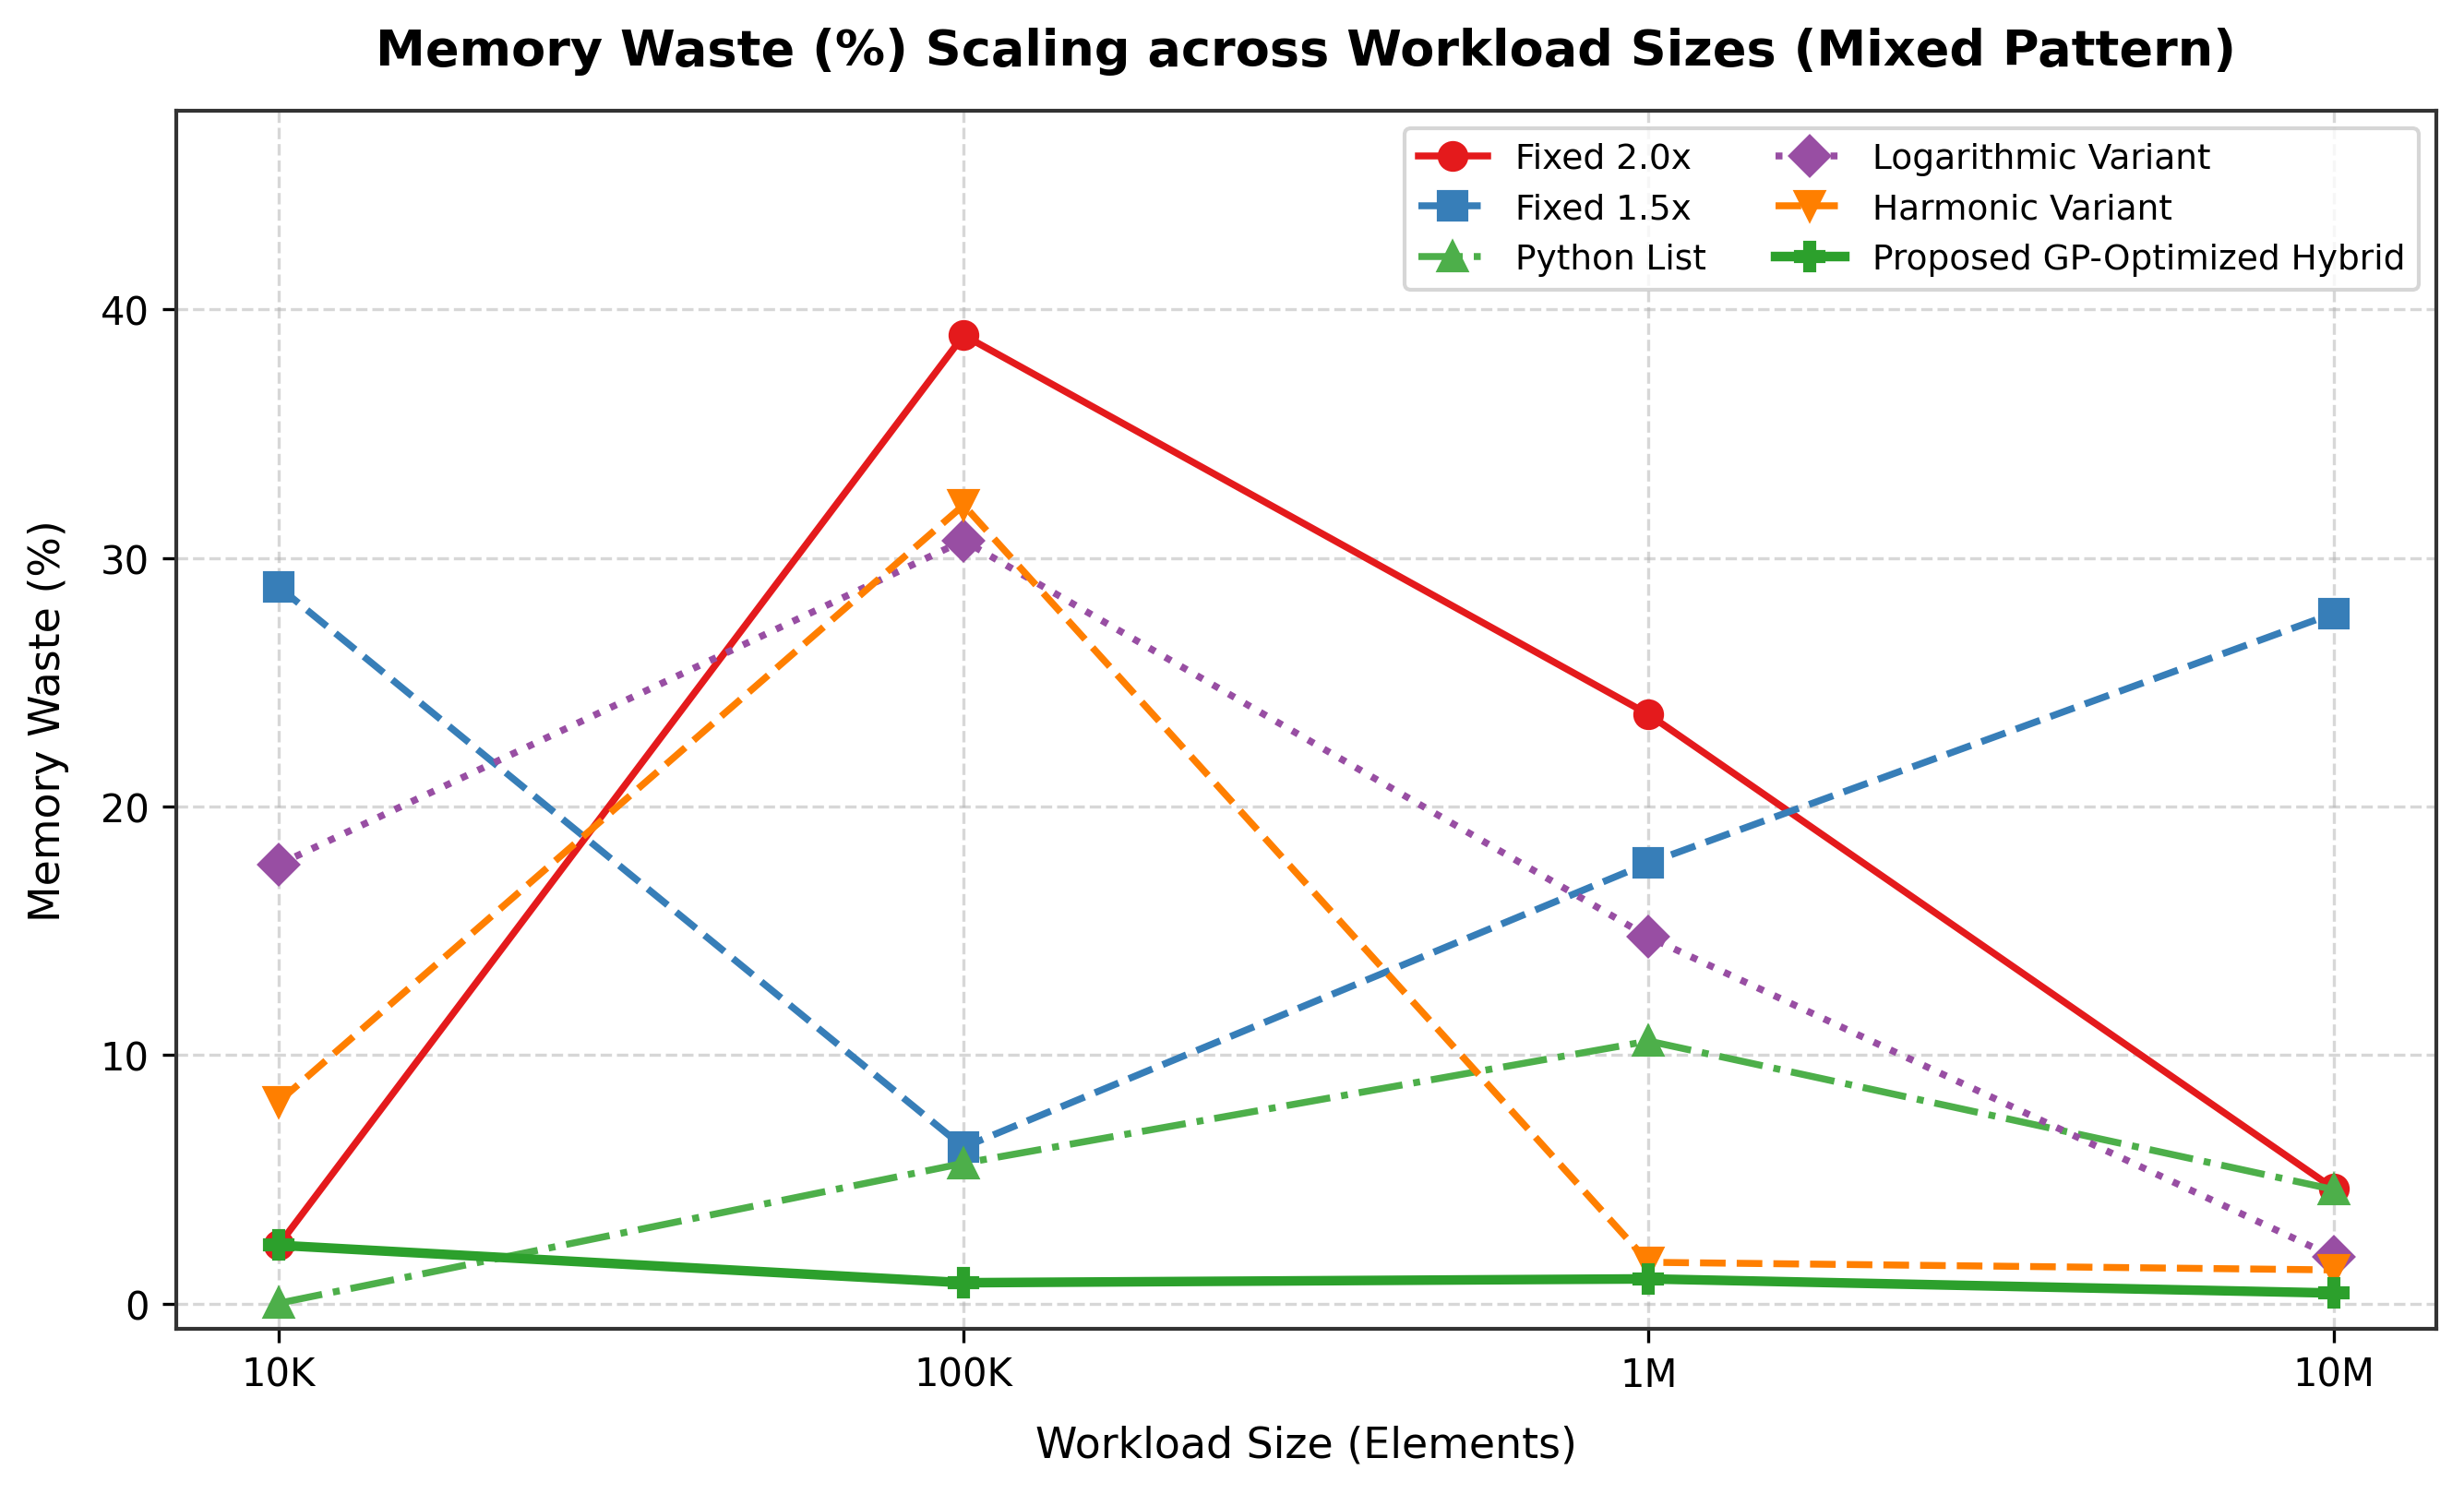
\includegraphics[width=0.95\linewidth]{fd_combined_workload_size_line.png}}
\caption{Memory waste (\%) vs.\ workload size under the mixed pattern.}
\label{fig:size_scaling}
\end{figure}

At $10^4$ elements, all strategies show low waste. As size scales to $10^7$ elements, Java 1.5x waste climbs fast, while doubling stays around 5\%. Tests across seven workload patterns shows our approach maintains near-zero waste across all scale points, showing size-independent efficiency by dropping growth toward $g_{\min}$ as velocity slows down in mature arrays.

Overall, our hybrid model cuts the cost score by 59.5\% compared to standard doubling ($J=0.64$). While exact runtime depends on language implementation details, memory waste and copy counts are platform-independent.

\section{Conclusion and Future Work}
We built workload-aware growth algorithm for dynamic arrays that replaces fixed expansion rules with a dynamic growth factor based on insertion velocity and resize history. Our hybrid function blends logarithmic and harmonic decay. Using GP-BO, we tuned the parameters to balance memory waste, copy operations, and runtime.

Tests across seven workload patterns shows our approach cuts memory waste by 90.9\% over 2.0x doubling, while matching the best copy count and resize frequency. Scaling tests confirm this spatial advantage works across large array sizes.

Next we plan to integrate this growth logic directly into CPython's \texttt{listobject.c} and C++ STL \texttt{std::vector}. We also plan to study online parameter tuning during application execution.

\begin{thebibliography}{26}
\bibitem{java_data_structures}
D.~E. Costa, A.~Andrzejak, J.~Seboek, and D.~Lo, ``Empirical Study of Usage and Performance of Java Collections,'' in \emph{Proc. 8th ACM/SPEC Int. Conf. Performance Engineering (ICPE)}, 2017, pp. 389--400.

\bibitem{time_space_complexity}
R.~E. Tarjan and U.~Zwick, ``Optimal Resizable Arrays,'' in \emph{Proc. 5th Symp. Simplicity in Algorithms (SOSA)}, 2023, pp. 1--10.

\bibitem{optimal_resizable}
A.~Brodnik, S.~Carlsson, E.~D. Demaine, J.~I. Munro, and R.~Sedgewick, ``Resizable Arrays in Optimal Time and Space,'' in \emph{Proc. 6th Int. Workshop Algorithms and Data Structures (WADS)}, 1999, pp. 37--48.

\bibitem{resizable_optimal_time_space}
P.~Bille, A.~R. Christiansen, M.~B. Ettienne, and I.~L. G{\o}rtz, ``Fast Dynamic Arrays,'' in \emph{Proc. 25th Annual European Symposium on Algorithms (ESA)}, 2017, pp. 16:1--16:14.

\bibitem{allocating_storage}
A.~L. Rosenberg, ``Allocating Storage for Extendible Arrays,'' \emph{Journal of the ACM}, vol. 21, no. 4, pp. 652--670, 1974.

\bibitem{managing_storage}
A.~L. Rosenberg, ``Managing Storage for Extendible Arrays,'' \emph{SIAM Journal on Computing}, vol. 4, no. 3, pp. 287--306, 1975.

\bibitem{fast_array}
J.~Katajainen, ``Worst-case-efficient Dynamic Arrays in Practice,'' in \emph{Proc. 15th Int. Symposium on Experimental Algorithms (SEA)}, 2016, pp. 202--217.

\bibitem{adaptive_packed}
M.~A. Bender, R.~Cole, E.~D. Demaine, and M.~Farach-Colton, ``Adaptive Packed Memory Array,'' \emph{ACM Transactions on Database Systems}, vol. 30, no. 4, pp. 110--128, 2005.

\bibitem{trends_adaptive}
H.~Singh and R.~M. Jha, ``Trends in Adaptive Array Processing,'' \emph{International Journal of Antennas and Propagation}, vol. 2012, pp. 1--11, 2012.

\bibitem{black_white_array}
Z.~G. Mou, ``Black-White Array: A New Data Structure for Dynamic Data Sets,'' \emph{arXiv preprint arXiv:cs/0409051}, pp. 1--15, 2004.

\bibitem{z_rays}
J.~B. Sartor, S.~M. Blackburn, D.~Frampton, M.~Hirzel, and K.~S. McKinley, ``Z-rays: Divide Arrays and Conquer Speed and Flexibility,'' in \emph{Proc. 31st ACM SIGPLAN Conf. Programming Language Design and Implementation (PLDI)}, 2010, pp. 406--417.

\bibitem{logarithmic_arrays}
R.~R. Hoogerwoord, ``A Logarithmic Implementation of Flexible Arrays,'' in \emph{Proc. 2nd International Conference on Mathematics of Program Construction (MPC)}, 1992, pp. 191--207.

\bibitem{lock_free_vector}
D.~Dechev, P.~Pirkelbauer, and B.~Stroustrup, ``Lock-Free Dynamically Resizable Arrays,'' in \emph{Proc. 10th International Conference on Principles of Distributed Systems (OPODIS)}, 2006, pp. 142--156.

\bibitem{persistent_arrays}
P.~F. Dietz, ``Fully Persistent Arrays,'' in \emph{Proc. 1st Workshop on Algorithms and Data Structures (WADS)}, 1989, pp. 67--74.

\bibitem{query_processing}
P.~Baumann, A.~Dehmel, P.~Furtado, R.~Ritsch, and N.~Widmann, ``The Multidimensional Database System RasDaMan,'' in \emph{Proc. 1998 ACM SIGMOD International Conference on Management of Data}, 1998, pp. 575--577.

\bibitem{cormen_algorithms}
T.~H. Cormen, C.~E. Leiserson, R.~L. Rivest, and C.~Stein, \emph{Introduction to Algorithms}, 4th~ed. Cambridge, MA, USA: MIT Press, 2022.

\bibitem{python_list_impl}
Python Software Foundation, ``CPython List Object Implementation,'' CPython Source Code, GitHub Repository, \texttt{listobject.c}, 2023.

\bibitem{practical_bayesian_opt}
J.~Snoek, H.~Larochelle, and R.~P. Adams, ``Practical Bayesian Optimization of Machine Learning Algorithms,'' in \emph{Proc. 25th International Conference on Neural Information Processing Systems (NIPS)}, 2012, pp. 2951--2959.

\bibitem{bayesian_opt_review}
B.~Shahriari, K.~Swersky, Z.~Wang, R.~P. Adams, and N.~de Freitas, ``Taking the Human Out of the Loop: A Review of Bayesian Optimization,'' \emph{Proceedings of the IEEE}, vol. 104, no. 1, pp. 148--175, 2016.

\bibitem{dynamic_storage_allocation}
P.~R. Wilson, M.~S. Johnstone, M.~Neely, and D.~Boles, ``Dynamic Storage Allocation: A Survey and Critical Review,'' in \emph{Proc. 1st International Workshop on Memory Management (IWMM)}, 1995, pp. 1--116.

\bibitem{reconsidering_custom_allocation}
E.~D. Berger, B.~G. Zorn, and K.~S. McKinley, ``Reconsidering Custom Memory Allocation,'' in \emph{Proc. 17th ACM SIGPLAN Conference on Object-Oriented Programming, Systems, Languages, and Applications (OOPSLA)}, 2002, pp. 1--12.

\bibitem{frigo_cache_oblivious}
M.~Frigo, C.~E. Leiserson, H.~Prokop, and S.~Ramachandran, ``Cache-Oblivious Algorithms,'' in \emph{Proc. 40th Annual Symposium on Foundations of Computer Science (FOCS)}, 1999, pp. 285--297.

\bibitem{python_malloc_impl}
Python Software Foundation, ``CPython Object Allocator Implementation,'' CPython Source Code, GitHub Repository, \texttt{obmalloc.c}, 2023.

\bibitem{scikit_optimize}
T.~Head, M.~Kumar, H.~Nahrstaedt, G.~Louppe, and I.~Shcherbatyi, ``scikit-optimize: Sequential model-based optimization in Python,'' Zenodo, \texttt{https://github.com/scikit-optimize/scikit-optimize}, 2018.

\bibitem{jones_ego}
D.~R. Jones, M.~Schonlau, and W.~J. Welch, ``Efficient Global Optimization of Expensive Black-Box Functions,'' \emph{Journal of Global Optimization}, vol. 13, no. 4, pp. 455--492, 1998.

\bibitem{hoard_allocator}
E.~D. Berger, K.~S. McKinley, R.~D. Blumofe, and P.~R. Wilson, ``Hoard: A Scalable Memory Allocator for Multithreaded Applications,'' in \emph{Proc. 9th International Conference on Architectural Support for Programming Languages and Operating Systems (ASPLOS)}, 2000, pp. 117--128.
\end{thebibliography}

\end{document}
